\documentclass[tikz,border=6pt]{standalone}
% Shared preamble for the CenterTask panel files (panel_a/b/c.tex).
% Edit colours and node styles here, once.
\usepackage{amsmath}
\usetikzlibrary{arrows.meta,positioning,calc}

% category colours as in ColorCategoryMap.m: 1=Short/Orange, 2=Mid/Green, 3=Long/Blue
\definecolor{catShort}{RGB}{243,178,132}
\definecolor{catMid}{RGB}{158,209,172}
\definecolor{catLong}{RGB}{157,188,234}

\tikzset{ctpanel/.style={
  font=\sffamily,
  band/.style={rounded corners=6pt, fill=black!7, draw=none, inner sep=8pt, minimum height=1.15cm},
  unit/.style={circle, fill=catMid!60, draw=none, minimum size=0.95cm, inner sep=0pt},
  flow/.style={-{Latex[length=2.2mm]}, line width=0.8pt},
  rowlab/.style={anchor=east, font=\sffamily\large},
  now/.style={fill=catShort!55, rounded corners=3pt, inner sep=3pt},
  stage/.style={rounded corners=6pt, fill=black!8, draw=none, inner sep=8pt, minimum height=1.2cm, align=center},
  target/.style={circle, minimum size=0.9cm, inner sep=0pt, draw=none, font=\sffamily\scriptsize, text=black!75},
  axis/.style={line width=0.6pt},
}}


% ---------------------------------------------------------------------
%  Pure iconography: the CUE frame (bar + centre hold + colour-cue dots)
%  in its 2-category and 3-category forms. No panel letter, no captions,
%  no timing/legend text -- just the two illustrative frames.
% ---------------------------------------------------------------------

\begin{document}
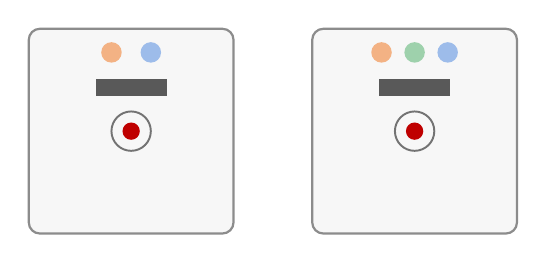
\begin{tikzpicture}[
  font=\sffamily,
  screen/.style={rounded corners=4pt, draw=black!45, line width=0.8pt, fill=black!3,
                 minimum width=2.6cm, minimum height=2.6cm},
  cursor/.style={circle, fill=red!75!black, draw=none, minimum size=2.2mm, inner sep=0pt},
  hold/.style={circle, draw=black!55, line width=0.7pt, fill=none},
  cuecirc/.style={circle, minimum size=2.6mm, inner sep=0pt},
]

\def\holdR{2.5mm}
\def\barW{9mm}
\def\barH{2.2mm}

% ---------- 2-category cue ----------
\begin{scope}[xshift=0cm]
  \node[screen] (A) at (0,0) {};
  \draw[hold] (A) circle (\holdR);
  \node[cursor] at (A) {};
  \fill[black!65] ($(A)+(0,0.55)$) ++(-\barW/2,-\barH/2) rectangle ++(\barW,\barH);
  \node[cuecirc, fill=catShort] at ($(A)+(-0.25,1.0)$) {};
  \node[cuecirc, fill=catLong]  at ($(A)+(0.25,1.0)$) {};
\end{scope}

% ---------- 3-category cue ----------
\begin{scope}[xshift=3.6cm]
  \node[screen] (B) at (0,0) {};
  \draw[hold] (B) circle (\holdR);
  \node[cursor] at (B) {};
  \fill[black!65] ($(B)+(0,0.55)$) ++(-\barW/2,-\barH/2) rectangle ++(\barW,\barH);
  \node[cuecirc, fill=catShort] at ($(B)+(-0.42,1.0)$) {};
  \node[cuecirc, fill=catMid]   at ($(B)+(0,1.0)$) {};
  \node[cuecirc, fill=catLong]  at ($(B)+(0.42,1.0)$) {};
\end{scope}

\end{tikzpicture}
\end{document}
